\documentclass[tikz,border=10pt]{standalone}
\usepackage[T1]{fontenc}
\usepackage{lmodern}
\usetikzlibrary{arrows.meta,backgrounds,calc}
\definecolor{blue}{HTML}{0072B2}
\definecolor{green}{HTML}{009E73}
\definecolor{orange}{HTML}{B44B00}
\definecolor{ink}{HTML}{243447}
\definecolor{gray}{HTML}{738294}
\tikzset{
 box/.style={draw=gray,rounded corners=3pt,text width=34mm,minimum height=14mm,align=center,text=ink,inner sep=5pt,font=\sffamily\small},
 actor/.style={box,text width=24mm,fill=white},
 component/.style={box,fill=blue!6},
 store/.style={box,fill=yellow!14},
 external/.style={box,fill=gray!7},
 panel/.style={fill=blue!2,draw=gray,rounded corners=5pt},
 flow/.style={-{Latex[length=2.5mm]},line width=1.25pt},
 run/.style={flow,draw=blue},
 again/.style={flow,draw=orange},
 grade/.style={flow,draw=green},
 relation/.style={draw=gray,dashed,line width=.85pt},
 label/.style={font=\sffamily\small,text=ink,align=center,fill=none,inner sep=2pt},
 heading/.style={font=\sffamily\bfseries,text=ink,anchor=west},
 title/.style={font=\sffamily\bfseries\Large,text=ink,anchor=west},
 note/.style={font=\sffamily\small,text=ink,anchor=west},
 every node/.append style={font=\sffamily}
}
\newcommand{\step}[2]{\tikz[baseline=(s.base)]\node[circle,fill=#1,text=white,inner sep=1.6pt,font=\sffamily\tiny\bfseries](s){#2};}

\begin{document}
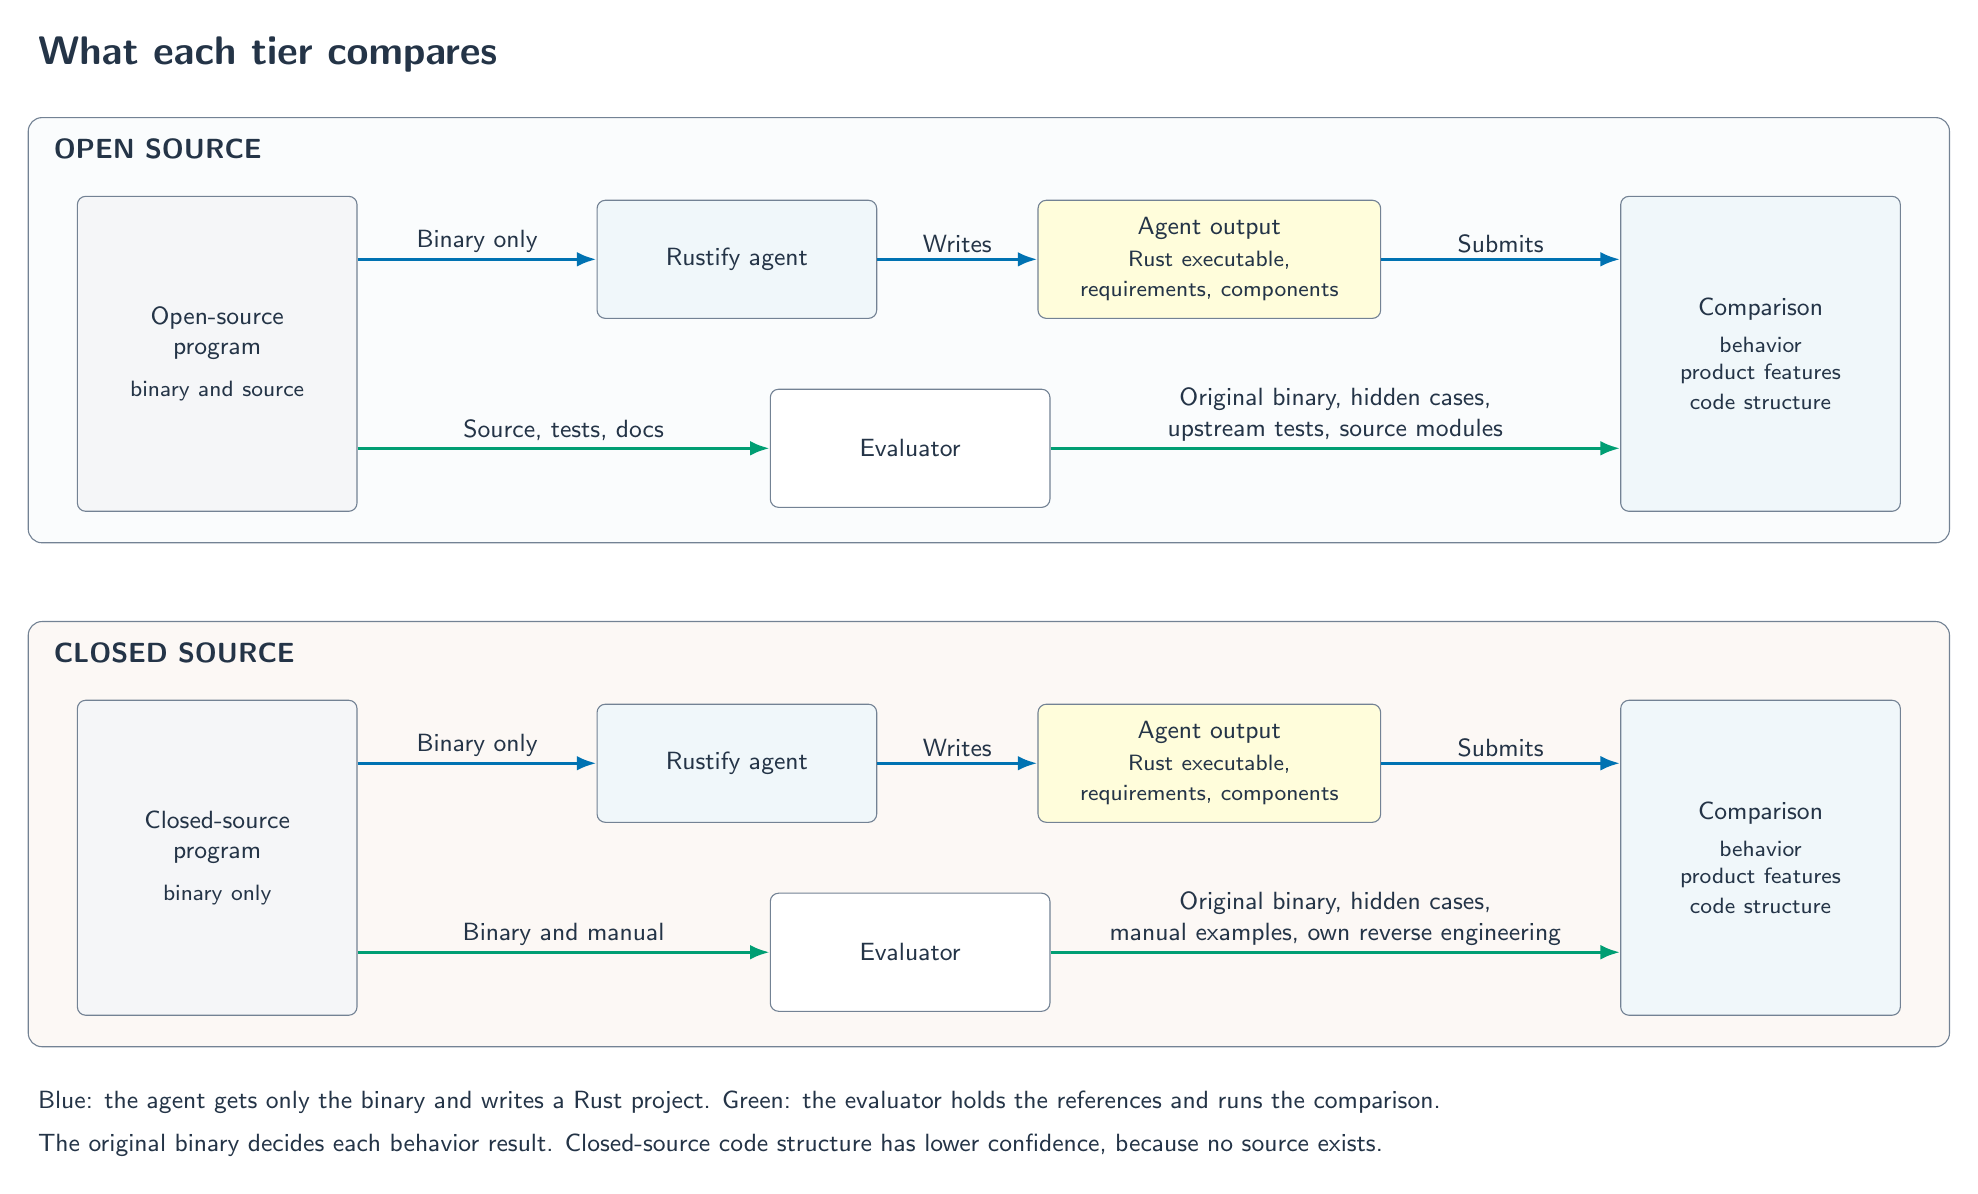
\begin{tikzpicture}[x=1cm,y=1cm]
 \tikzset{part/.style={box,text width=32mm,minimum height=15mm},
  software/.style={part,fill=gray!7,minimum height=40mm},
  output/.style={part,fill=yellow!14,text width=40mm},
  comparison/.style={part,fill=blue!6,minimum height=40mm}}
 \node[title] at (-0.4,8.4) {What each tier compares};
 \begin{scope}[on background layer]
  \filldraw[panel] (-0.4,2.2) rectangle (24.0,7.6);
  \filldraw[fill=orange!4,draw=gray,rounded corners=5pt] (-0.4,-4.2) rectangle (24.0,1.2);
 \end{scope}
 \foreach \y/\tier/\software/\given/\references in {
  4.6/OPEN SOURCE/{Open-source\\program\\[4pt]\footnotesize binary and source}/{Source, tests, docs}/{Original binary, hidden cases,\\upstream tests, source modules},
  -1.8/CLOSED SOURCE/{Closed-source\\program\\[4pt]\footnotesize binary only}/{Binary and manual}/{Original binary, hidden cases,\\manual examples, own reverse engineering}} {
  \node[heading] at (-0.2,\y+2.6) {\tier};
  \node[software] (software) at (2.0,\y) {\software};
  \node[component,part] (agent) at (8.6,\y+1.2) {Rustify agent};
  \node[output] (output) at (14.6,\y+1.2) {Agent output\\[2pt]\footnotesize Rust executable,\\\footnotesize requirements, components};
  \node[actor,part] (evaluator) at (10.8,\y-1.2) {Evaluator};
  \node[comparison] (compare) at (21.6,\y) {Comparison\\[4pt]\footnotesize behavior\\\footnotesize product features\\\footnotesize code structure};
  \draw[run] (software.east |- agent.west) -- node[label,above]{Binary only} (agent.west);
  \draw[run] (agent.east) -- node[label,above]{Writes} (output.west);
  \draw[run] (output.east) -- node[label,above]{Submits} (compare.west |- output.east);
  \draw[grade] (software.east |- evaluator.west) -- node[label,above]{\given} (evaluator.west);
  \draw[grade] (evaluator.east) -- node[label,above]{\references} (compare.west |- evaluator.east);
 }
 \node[note] at (-0.4,-4.9) {Blue: the agent gets only the binary and writes a Rust project. Green: the evaluator holds the references and runs the comparison.};
 \node[note] at (-0.4,-5.45) {The original binary decides each behavior result. Closed-source code structure has lower confidence, because no source exists.};
\end{tikzpicture}
\end{document}
